% !TEX root = ../main.tex
% 本文件由 build-tex.sh 从 14-DSP指南-第14章中译.md 生成，改内容请改 md 后重新生成

\chapter{数字滤波器入门}\label{ch-14}

数字滤波器(digital filter)有两大用途：(1) 把混在一起的信号分开；(2)
把以某种方式失真了的信号复原。模拟（电子）滤波器也能完成同样的任务，但数字滤波器能取得好得多的效果。接下来的七章会介绍并比较最常用的数字滤波器。这一章是入门，介绍学习每种滤波器时应该关注哪些参数。

\section{滤波器基础}

数字滤波器是 DSP 中非常重要的一部分。事实上，它们出色的性能正是 DSP
变得如此流行的关键原因之一。如引言所说，滤波器有两个用途：信号分离(signal
separation)和信号复原(signal
restoration)。当一个信号被干扰、噪声或其他信号污染时，就需要信号分离。例如，设想一台测量胎儿在子宫内心脏电活动（心电图，EKG）的设备。原始信号很可能被母亲的呼吸和心跳破坏。可以用滤波器把这些信号分开，以便分别分析。

当信号以某种方式失真时，就要用信号复原。例如，用劣质设备录的音频可以经过滤波，更好地还原当时真实的声音。另一个例子是给对焦不准的镜头或抖动的相机拍到的图像去模糊。

这些问题既可以用模拟滤波器解决，也可以用数字滤波器解决。哪个更好？模拟滤波器便宜、快速，在幅度和频率上都有很大的动态范围(dynamic
range)。相比之下，数字滤波器能达到的性能水平要高得多。例如，第 16
章介绍的一个低通数字滤波器，从直流到 1000 赫兹的增益是 1 ± 0.0002，1001
赫兹以上频率的增益小于 0.0002。整个过渡只发生在 1
赫兹之内。别指望运放电路能做到这样！数字滤波器的性能可以比模拟滤波器好上千倍。这让解决滤波问题的思路发生了巨大变化。用模拟滤波器时，重点是应对电子器件的局限，比如电阻和电容的精度与稳定性。相比之下，数字滤波器好到它本身的性能常常可以不予考虑，重点转移到信号本身的局限，以及处理这些信号的理论问题上。

在 DSP 中，人们常说滤波器的输入和输出信号处在时域(time
domain)。这是因为信号通常是按相等的时间间隔采样得到的。但这不是唯一的采样方式。第二常见的方式是按相等的空间间隔采样。例如，设想沿飞机机翼的长度方向每隔一厘米装一个应变传感器，同时读取这一排传感器的读数。其他的域也有可能，但时间和空间是迄今为止最常见的。在
DSP
中看到''时域''这个词时，记住它可能真的指随时间采集的样本，也可能泛指采样所在的任何域。

如图 14-1 所示，每个线性滤波器都有一个冲激响应(impulse
response)、一个阶跃响应(step response)和一个频率响应(frequency
response)。这三者每一个都包含了关于滤波器的完整信息，只是形式不同。只要给定其中一个，另外两个就确定了，可以直接算出来。这三种表示都很重要，因为它们描述了滤波器在不同情形下会怎样反应。

实现数字滤波器最直接的方法，是把输入信号与数字滤波器的冲激响应卷积。所有可能的线性滤波器都能用这种方式做出来。（这应该是显然的。如果你不觉得显然，那你大概还不具备理解这一部分滤波器设计的基础。试着复习一下前面关于
DSP
基础的部分。）当冲激响应这样使用时，滤波器设计者给它起了个专门的名字：滤波器核(filter
kernel)。

做数字滤波器还有另一种方法，叫递归(recursion)。用卷积实现滤波器时，输出中的每个采样都是对输入采样加权后相加得到的。递归滤波器(recursive
filter)是这种做法的扩展：除了用输入中的点，还用之前已经算出的输出值。递归滤波器不用滤波器核，而是用一组递归系数(recursion
coefficients)来定义。这种方法会在第 19
章详细讨论。眼下的要点是：所有线性滤波器都有冲激响应，即使你不用它来实现滤波器。要求出递归滤波器的冲激响应，只要输入一个冲激，看看输出什么就行了。递归滤波器的冲激响应由幅度按指数衰减的正弦波组成。原则上，这使它们的冲激响应无限长。不过，幅度最终会降到系统的舍入噪声以下，剩下的采样就可以忽略。由于这个特点，递归滤波器也叫无限冲激响应(Infinite
Impulse Response)滤波器，即 IIR
滤波器。相比之下，用卷积实现的滤波器叫有限冲激响应(Finite Impulse
Response)滤波器，即 FIR 滤波器。

\begin{figure}[htbp]
\centering
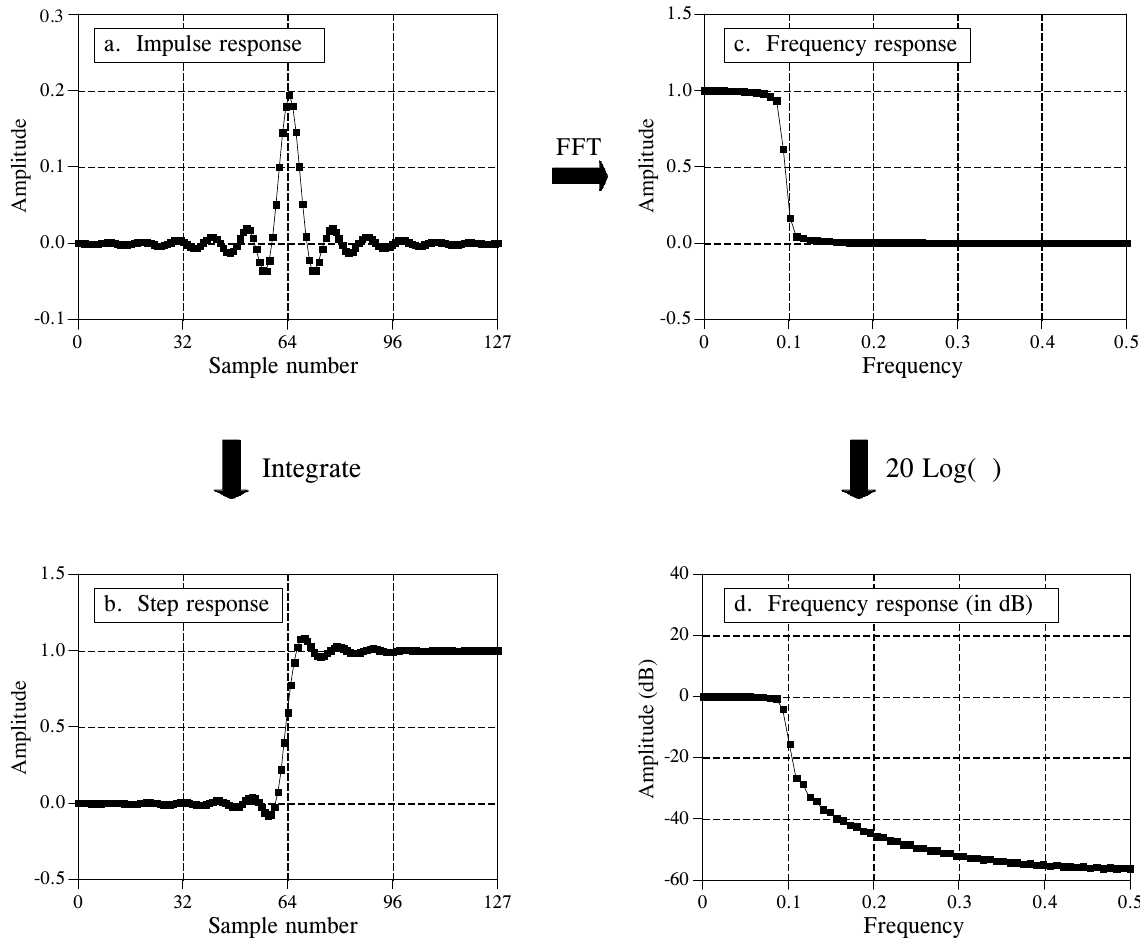
\includegraphics[width=0.950\linewidth,height=0.8\textheight,keepaspectratio]{assets/ch14/fig14-01.png}
\caption*{\textbf{图 14-1　滤波器的参数。}
每个线性滤波器都有冲激响应、阶跃响应和频率响应。阶跃响应 (b)
可以通过对冲激响应 (a)
做离散积分求得。频率响应可以用快速傅里叶变换（FFT）从冲激响应求得，既可以用线性刻度显示
(c)，也可以用分贝显示 (d)。 （a. Impulse response = 冲激响应；b. Step
response = 阶跃响应；c.~Frequency response = 频率响应；d.~Frequency
response (in dB) = 频率响应（分贝）。箭头：FFT；Integrate = 积分；20
Log( ) = 取 20 倍对数。Amplitude = 幅度，Amplitude (dB) =
幅度（分贝），Sample number = 采样序号，Frequency = 频率。）}
\end{figure}

你已经知道，冲激响应是输入为冲激时系统的输出。同样，阶跃响应是输入为阶跃(step)时的输出（阶跃也叫边沿(edge)，阶跃响应也叫边沿响应(edge
response)）。由于阶跃是冲激的积分，阶跃响应就是冲激响应的积分。这提供了两种求阶跃响应的方法：(1)
把阶跃波形送进滤波器，看输出什么；(2)
对冲激响应积分。（数学上严格地说：积分用于连续信号，而离散积分，即累加和，用于离散信号。）频率响应可以通过对冲激响应做
DFT（用 FFT
算法）求得，本章后面会复习这一点。频率响应可以画在线性纵轴上，如
(c)；也可以画在对数刻度（分贝）上，如
(d)。线性刻度最适合显示通带纹波和滚降，而要显示阻带衰减就需要分贝刻度。

记不清分贝了？这里快速复习一下。一贝尔(bel，为纪念亚历山大·格雷厄姆·贝尔而得名)表示功率变化了十倍。例如，一个放大倍数为
3 贝尔的电子电路，输出信号的功率是输入的 10 × 10 × 10 = 1000
倍。一分贝(decibel，dB)是十分之一贝尔。因此，−20dB、−10dB、0dB、10dB 和
20dB 分别对应功率比 0.01、0.1、1、10 和
100。换句话说，每十分贝表示功率变化了十倍。

问题在于：你通常想处理的是信号的幅度，而不是功率。例如，设想一个增益为
20dB 的放大器。按定义，这意味着信号的功率增大了 100
倍。由于幅度与功率的平方根成正比，输出的幅度是输入的 10 倍。20dB
在功率上意味着 100 倍，在幅度上却只意味着 10
倍。每二十分贝表示幅度变化了十倍。写成公式：

\textbf{公式
14-1}　分贝的定义。分贝是表示两个信号之比的一种方式。功率之比（P₁ 和
P₂）与幅度之比（A₁ 和 A₂）用的公式不同。

\[\text{dB} = 10\log_{10}\frac{P_2}{P_1}\]

\[\text{dB} = 20\log_{10}\frac{A_2}{A_1}\]

上面的公式用的是以 10 为底的对数，但许多计算机语言只提供以 e
为底的对数函数（自然对数，写作 \(\log_e x\) 或
\(\ln x\)）。把上面的公式改一下就能用自然对数：\(\text{dB} = 4.342945\,\log_e(P_2/P_1)\)
和 \(\text{dB} = 8.685890\,\log_e(A_2/A_1)\)。

既然分贝是表示两个信号之比的方式，它就非常适合描述系统的增益，即输出信号与输入信号之比。不过，工程师也用分贝来标定单个信号的幅度（或功率），办法是把它与某个标准作参照。例如，dBV
表示以 1 伏有效值(rms)的信号为参照。同样，dBm 表示以在 600 欧负载上产生
1 毫瓦功率的信号为参照（约 0.78 伏有效值）。

如果关于分贝你别的什么都记不住，就记住两件事。第一，−3dB 表示幅度降到
0.707（因而功率降到 0.5）。第二，背下下面这些分贝与幅度比之间的换算：

{\def\LTcaptype{none} % do not increment counter
\begin{longtable}[]{@{}rr@{}}
\toprule\noalign{}
分贝 & 幅度比 \\
\midrule\noalign{}
\endhead
\bottomrule\noalign{}
\endlastfoot
60dB & 1000 \\
40dB & 100 \\
20dB & 10 \\
0dB & 1 \\
−20dB & 0.1 \\
−40dB & 0.01 \\
−60dB & 0.001 \\
\end{longtable}
}

\section{信息在信号中是怎样表示的}

任何 DSP
任务中最重要的部分，是弄懂信息是怎样包含在你所处理的信号中的。信息包含在信号中的方式有很多种，人造信号尤其如此。比如，想想人们设计出的各种调制方案：调幅(AM)、调频(FM)、单边带(single-sideband)、脉冲编码调制(pulse-code
modulation)、脉宽调制(pulse-width
modulation)等等，不胜枚举。幸运的是，在自然产生的信号中，常见的信息表示方式只有两种。我们把它们叫做：在时域中表示的信息，和在频域中表示的信息。

在时域中表示的信息，描述的是某件事什么时候发生、发生的幅度有多大。例如，设想一个研究太阳光输出的实验。光输出每秒测量并记录一次。信号中的每个采样都表明那一刻正在发生什么，以及事件的强度。如果发生了一次太阳耀斑，信号会直接给出它发生的时间、持续时长、随时间的发展等信息。每个采样所含的信息无需参照其他采样就能解读。即使你只有这个信号的一个采样，也仍然对所测的东西有所了解。这是信息包含在信号中最简单的方式。

相比之下，在频域中表示的信息更为间接。我们宇宙中的许多事物都呈现周期运动。例如，用指甲敲一下酒杯，它会振动，发出清脆的响声；落地钟的钟摆来回摆动；恒星和行星绕自身的轴自转、又相互绕转，等等。测量这种周期运动的频率、相位和幅度，往往能获得关于产生这种运动的系统的信息。假设我们对敲响的酒杯发出的声音采样。周期振动的基频和谐波与材料的质量和弹性有关。单独一个采样本身不含有任何关于周期运动的信息，因而也不含有任何关于酒杯的信息。信息包含在信号中许多点之间的关系里。

这就引出了阶跃响应和频率响应的重要性。阶跃响应描述了在时域中表示的信息被系统怎样改变。而频率响应展示了在频域中表示的信息被怎样改变。这个区别在滤波器设计中至关重要，因为不可能让一个滤波器同时在这两种应用中都达到最优。时域性能好，就会导致频域性能差，反之亦然。如果你设计的滤波器是要去除心电图信号中的噪声（信息在时域中表示），阶跃响应就是重要参数，频率响应则无关紧要。如果你的任务是为助听器设计数字滤波器（信息在频域中），频率响应就是一切，阶跃响应则无所谓。下面来看看是什么让一个滤波器在时域或频域应用中达到最优。

\section{时域参数}

为什么时域滤波器如此关注阶跃响应，可能并不显而易见。你也许会问，为什么重要参数不是冲激响应？答案在于人的大脑理解和处理信息的方式。记住，阶跃响应、冲激响应和频率响应包含的信息完全相同，只是排列方式不同。阶跃响应之所以在时域分析中有用，是因为它契合人看待信号中所含信息的方式。

例如，假设给你一个来历不明的信号，让你分析。你做的第一件事，就是把信号划分成特征相似的若干区域。你没法不这么做，你的大脑会自动这么做。有些区域可能很平滑，有些可能有很大的幅度峰值，有些可能噪声很多。这种分段是通过找出区域之间的分界点完成的。这正是阶跃函数(step
function)发挥作用的地方。阶跃函数是表示两个不同区域之间分界的最纯粹的方式。它可以标记一个事件何时开始，或者何时结束。它告诉你左边的东西在某种程度上与右边的东西不同。这就是人脑看待时域信息的方式：一组阶跃函数把信息划分成特征相似的区域。而阶跃响应之所以重要，是因为它描述了这些分界线被滤波器怎样改变。

滤波器设计中重要的阶跃响应参数如图 14-2
所示。要分辨信号中的事件，阶跃响应的持续时间必须短于事件之间的间隔。这就要求阶跃响应尽可能地快（这是
DSP 的行话），如图 (a) 和 (b)
所示。标定上升时间(risetime，又一个行话)最常用的方法，是给出幅度从 10\%
到 90\%
之间的采样数。为什么不能总是做到非常快的上升时间？原因很多：降低噪声、数据采集系统固有的限制、避免混叠等等。

\begin{figure}[htbp]
\centering
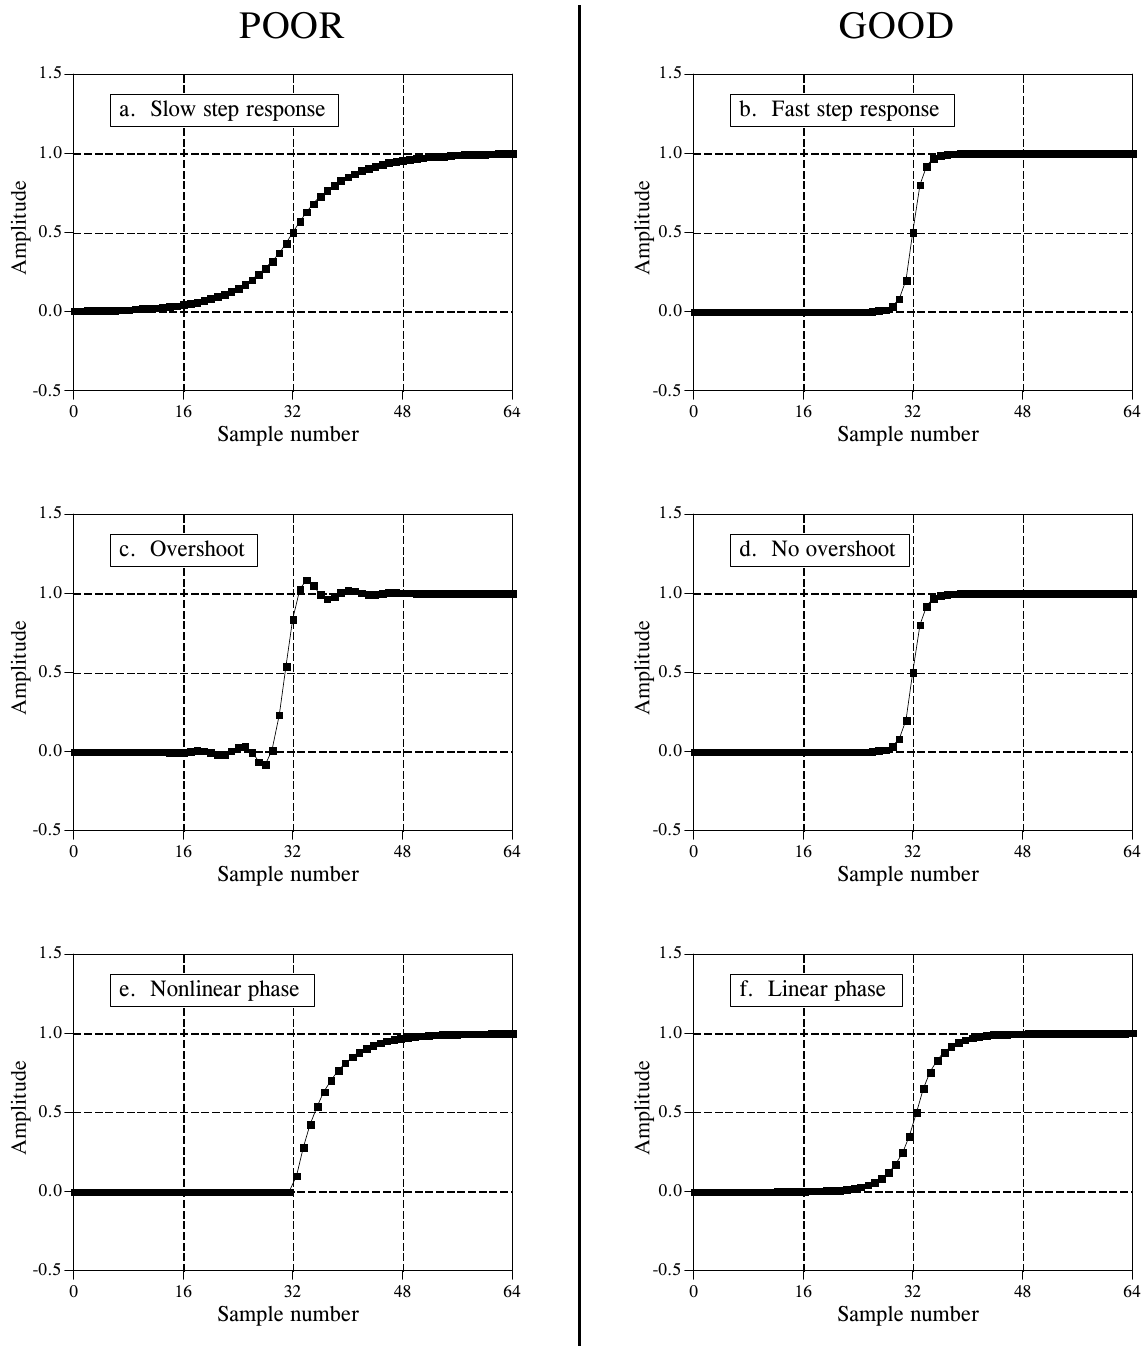
\includegraphics[width=0.954\linewidth,height=0.8\textheight,keepaspectratio]{assets/ch14/fig14-02.png}
\caption*{\textbf{图 14-2　评价时域性能的参数。}
阶跃响应用来衡量滤波器在时域中的表现。有三个参数很重要：(1)
过渡速度（上升时间），见 (a) 和 (b)；(2) 过冲，见 (c) 和 (d)；(3)
相位线性（阶跃上下两半的对称性），见 (e) 和 (f)。 （POOR = 差，GOOD =
好；a. Slow step response = 慢的阶跃响应；b. Fast step response =
快的阶跃响应；c.~Overshoot = 过冲；d.~No overshoot = 无过冲；e.
Nonlinear phase = 非线性相位；f.~Linear phase = 线性相位。Amplitude =
幅度，Sample number = 采样序号。）}
\end{figure}

图 (c) 和 (d)
展示了下一个重要参数：阶跃响应中的过冲(overshoot)。过冲一般必须消除，因为它改变了信号中采样的幅度，这是对时域中所含信息的一种根本性失真。这可以归结为一个问题：你在信号中看到的过冲，是来自你要测量的东西，还是来自你用的滤波器？

最后，人们常常希望阶跃响应的上半部分与下半部分对称，如 (e) 和 (f)
所示。需要这种对称性，才能让上升沿和下降沿看起来一样。这种对称叫线性相位(linear
phase)，因为频率响应的相位是一条直线（第 19
章讨论）。务必理解这三个参数，它们是评价时域滤波器的关键。

\section{频域参数}

图 14-3
展示了四种基本的频率响应。这些滤波器的目的，是让某些频率原封不动地通过，同时完全挡住另一些频率。通带(passband)指被通过的那些频率，阻带(stopband)包含被挡住的那些频率，过渡带(transition
band)在两者之间。滚降(roll-off)快，意味着过渡带非常窄。通带与过渡带的分界叫截止频率(cutoff
frequency)。在模拟滤波器设计中，截止频率通常定义为幅度降到 0.707（即
−3dB）的位置。数字滤波器的标准化程度没那么高，常见到把幅度降到
99\%、90\%、70.7\% 和 50\% 的位置定义为截止频率。

\begin{figure}[htbp]
\centering
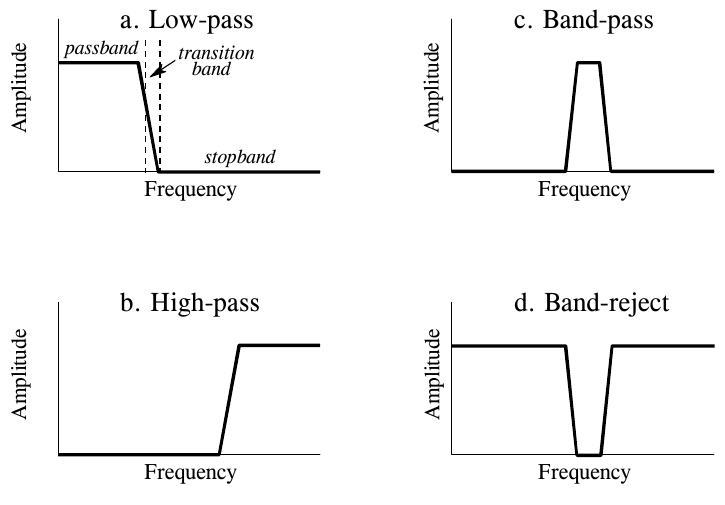
\includegraphics[width=0.604\linewidth,height=0.8\textheight,keepaspectratio]{assets/ch14/fig14-03.png}
\caption*{\textbf{图 14-3　四种常见的频率响应。}
频域滤波器一般用来让某些频率通过（通带），同时挡住另一些频率（阻带）。最常见的四种响应是：低通、高通、带通和带阻。
（a. Low-pass = 低通；b. High-pass = 高通；c.~Band-pass =
带通；d.~Band-reject = 带阻；passband = 通带，transition band =
过渡带，stopband = 阻带。Amplitude = 幅度，Frequency =
频率。原书这段图注排在图的左侧，裁图时已去掉，译文见上。）}
\end{figure}

图 14-4
展示了衡量滤波器频域性能的三个参数。要分开靠得很近的频率，滤波器必须滚降快，如
(a) 和 (b)
所示。要让通带频率原封不动地通过滤波器，就必须没有通带纹波(passband
ripple)，如 (c) 和 (d)
所示。最后，要充分挡住阻带频率，就需要良好的阻带衰减(stopband
attenuation)，如 (e) 和 (f) 所示。

\begin{figure}[htbp]
\centering
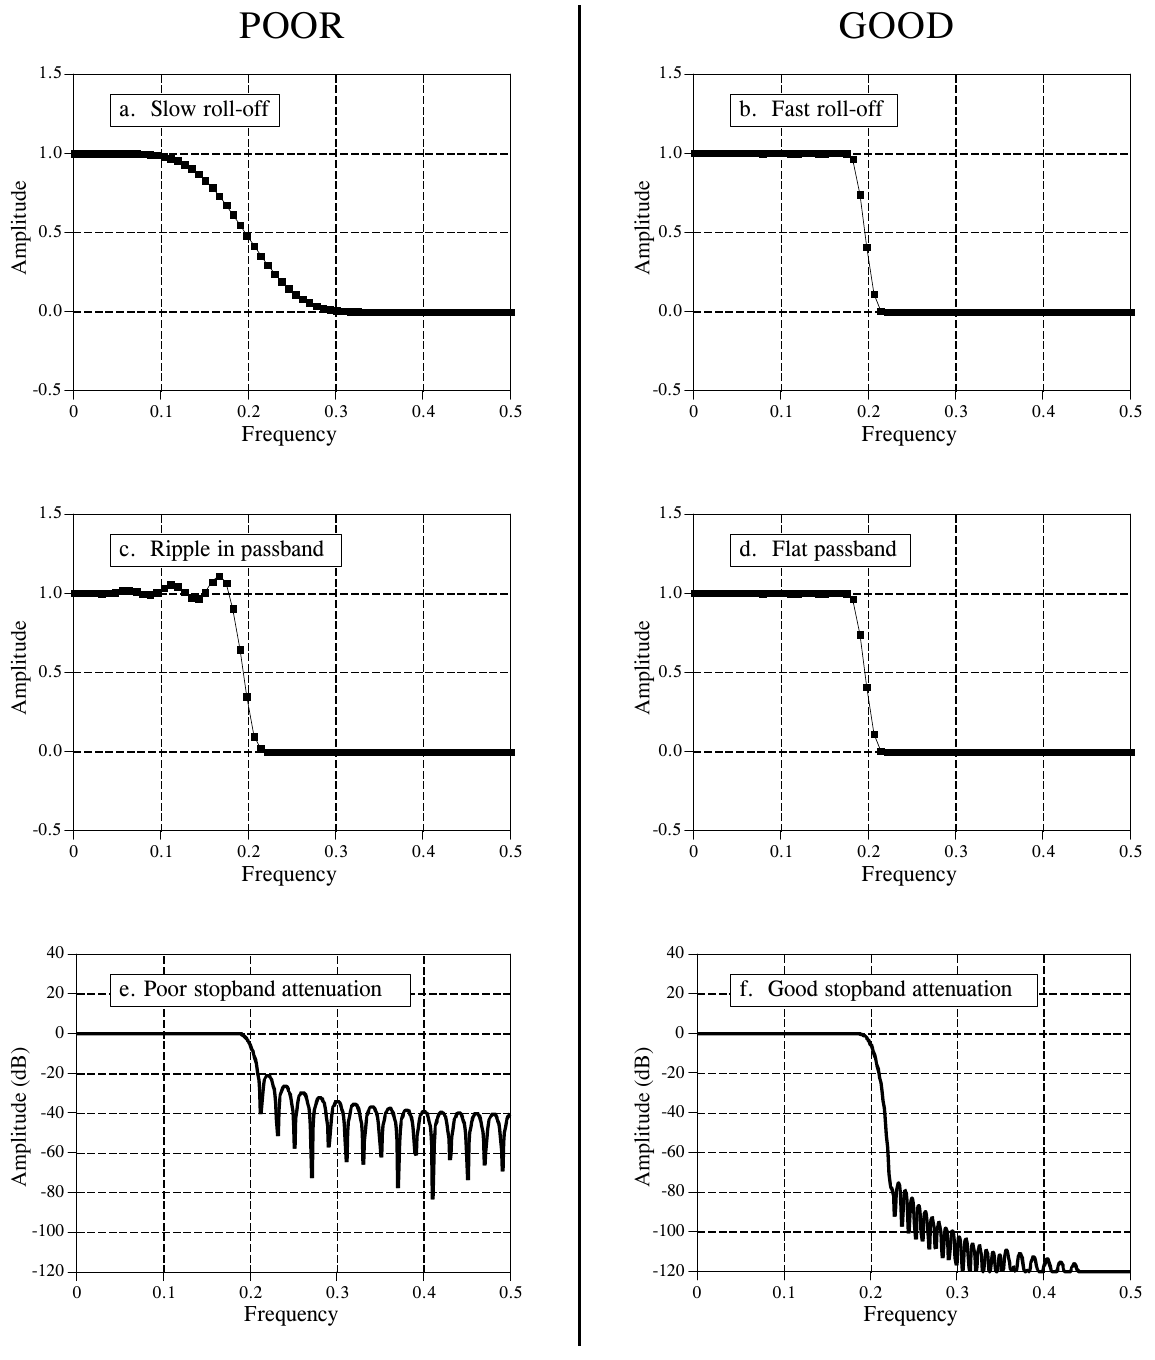
\includegraphics[width=0.963\linewidth,height=0.8\textheight,keepaspectratio]{assets/ch14/fig14-04.png}
\caption*{\textbf{图 14-4　评价频域性能的参数。}
图中的频率响应都是低通滤波器的。有三个参数很重要：(1) 滚降的陡峭程度，见
(a) 和 (b)；(2) 通带纹波，见 (c) 和 (d)；(3) 阻带衰减，见 (e) 和 (f)。
（POOR = 差，GOOD = 好；a. Slow roll-off = 滚降慢；b. Fast roll-off =
滚降快；c.~Ripple in passband = 通带有纹波；d.~Flat passband =
通带平坦；e. Poor stopband attenuation = 阻带衰减差；f.~Good stopband
attenuation = 阻带衰减好。Amplitude = 幅度，Amplitude (dB) =
幅度（分贝），Frequency = 频率。）}
\end{figure}

为什么这些参数里没有一个和相位有关？第一，在大多数频域应用中，相位并不重要。例如，音频信号的相位几乎完全是随机的，不含多少有用的信息。第二，如果相位很重要，做出相位响应完美的数字滤波器也非常容易，即所有频率通过滤波器时相移都为零（同样在第
19 章讨论）。相比之下，模拟滤波器在这方面糟糕透顶。

前面几章讲过 DFT
怎样把系统的冲激响应转换成频率响应。这里简单复习一下。计算 DFT
最快的方法是用第 12 章介绍的 FFT 算法。从一个 N 点长的滤波器核出发，FFT
算出的频谱由 N 点实部和 N 点虚部组成。FFT 实部和虚部中只有第 0 到第 N/2
个采样含有有用的信息，其余的点是重复的（负频率），可以忽略。由于实部和虚部人很难看懂，通常把它们转换成第
8 章介绍的极坐标形式。这就得到幅度信号和相位信号，各自从第 0 个采样到第
N/2 个采样（即每个信号有 N/2 + 1 个采样）。例如，256
点的冲激响应会得到从第 0 点到第 128 点的频率响应。第 0
个采样代表直流，即零频率；第 128
个采样代表采样率的一半。记住，采样数据中不可能出现高于采样率一半的频率。

用来表示冲激响应的采样数可以任意多。例如，假设你想求一个由 80
个点组成的滤波器核的频率响应。由于 FFT 只能处理长度为 2
的幂的信号，你需要给信号补 48 个零，使它长 128
个采样。补零不会改变冲激响应。要理解为什么，想想输入信号与系统冲激响应卷积时，这些补上的零会怎样：它们在卷积中直接消失，不影响结果。

更进一步，你可以给冲激响应补很多零，让它长达比如 256、512 或 1024
点。重要的一点是：冲激响应越长，频率响应中数据点的间距就越密。也就是说，在直流到采样率一半之间分布的采样更多。推到极致，如果给冲激响应补无穷多个零，频率响应中的数据点就无限接近，成为一条连续的线。换句话说，滤波器的频率响应实际上是直流到采样率一半之间的一个连续信号，DFT
的输出是对这条连续曲线的采样。计算滤波器的频率响应时，冲激响应该取多长？第一个念头可以试
N = 1024，但如果需要（比如分辨率不够或计算时间太长），别怕改。

记住，本章讨论的''好''与''坏''参数只是笼统的概括。许多信号并不能整整齐齐地归入某一类。例如，想想一个被
60
赫兹干扰污染的心电图信号。信息编码在时域中，但干扰最好在频域中处理。这种应用的最佳设计必然要有所取舍，而且可能和本章的常规观点相悖。记住教育的头号法则：书上的一段话并不是让你停止思考的许可证。

\section{高通、带通和带阻滤波器}

高通(high-pass)、带通(band-pass)和带阻(band-reject)滤波器的设计方法，是先设计一个低通(low-pass)滤波器，再把它转换成需要的响应。正因为如此，大多数关于滤波器设计的讨论只举低通滤波器的例子。从低通到高通的转换有两种方法：频谱反转(spectral
inversion)和频谱翻转(spectral reversal)。两种方法同样有用。

图 14-5 是频谱反转的一个例子。图 (a) 是一个叫加窗 sinc(windowed-sinc，第
16 章的主题)的低通滤波器核。这个滤波器核长 51
点，不过很多采样的值非常小，在这张图里看上去像是零。对应的频率响应如 (b)
所示，是给滤波器核补 13 个零、做 64 点 FFT
得到的。把低通滤波器核变成高通滤波器核要做两件事：第一，把滤波器核中每个采样的符号取反；第二，在对称中心的采样上加一。这样就得到
(c) 中的高通滤波器核，其频率响应如 (d)
所示。频谱反转把频率响应上下翻转，通带变成阻带，阻带变成通带。换句话说，它把滤波器从低通变成高通、高通变成低通、带通变成带阻、或者带阻变成带通。

\begin{figure}[htbp]
\centering
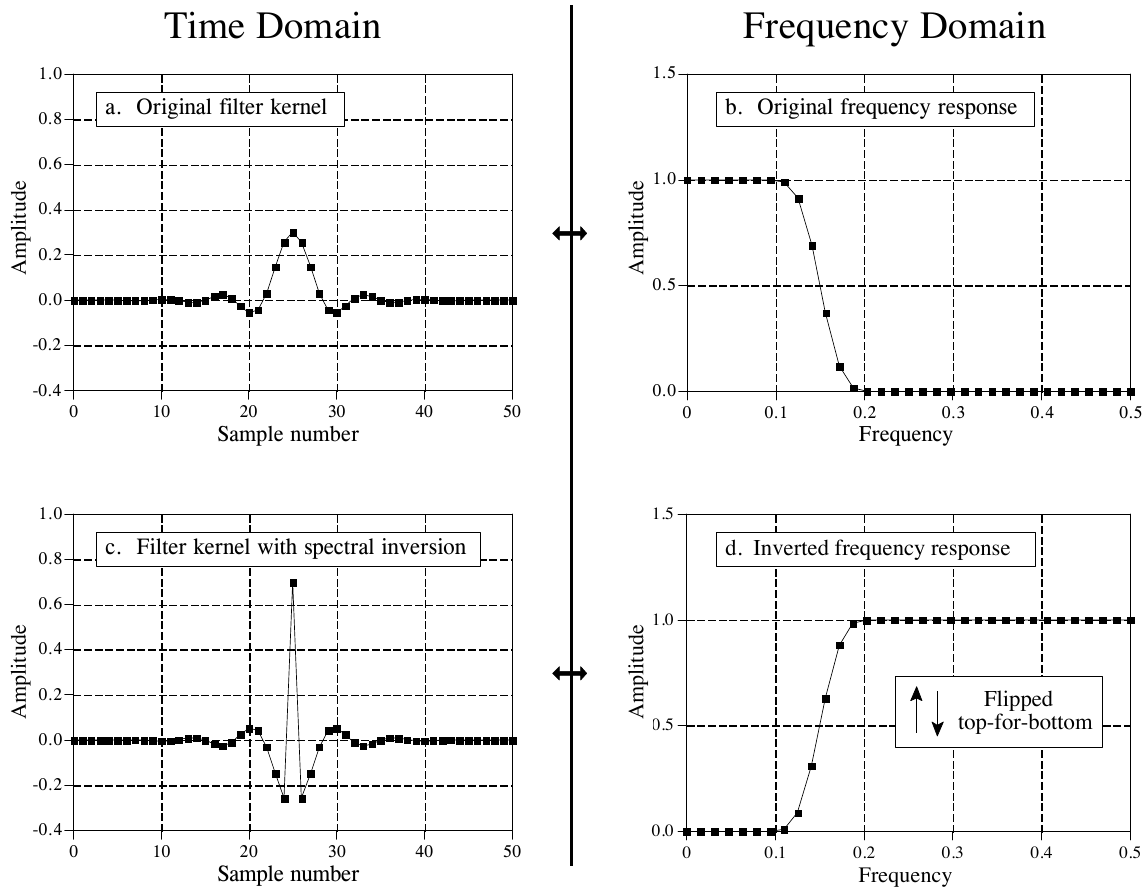
\includegraphics[width=0.954\linewidth,height=0.8\textheight,keepaspectratio]{assets/ch14/fig14-05.png}
\caption*{\textbf{图 14-5　频谱反转的例子。} (a) 中低通滤波器核的频率响应如 (b)
所示。把 (a)
中每个采样的符号取反，再在对称中心的采样上加一，就得到高通滤波器核
(c)。时域中的这一操作使频谱反转（即上下翻转），得到 (d)
所示的高通频率响应。 （Time Domain = 时域，Frequency Domain = 频域；a.
Original filter kernel = 原滤波器核；b. Original frequency response =
原频率响应；c.~Filter kernel with spectral inversion =
频谱反转后的滤波器核；d.~Inverted frequency response =
反转后的频率响应；Flipped top-for-bottom = 上下翻转。Amplitude =
幅度，Sample number = 采样序号，Frequency = 频率。）}
\end{figure}

图 14-6 说明了为什么时域中的这两步修改会使频谱反转。在 (a) 中，输入信号
x{[}n{]} 同时送入两个并联的系统。其中一个是低通滤波器，冲激响应为
h{[}n{]}。另一个对信号什么都不做，因此其冲激响应是一个冲激函数
δ{[}n{]}。总输出 y{[}n{]}
等于全通系统的输出减去低通系统的输出。由于低频成分从原信号中被减掉了，输出中只剩下高频成分。这样就构成了一个高通滤波器。

\begin{figure}[htbp]
\centering
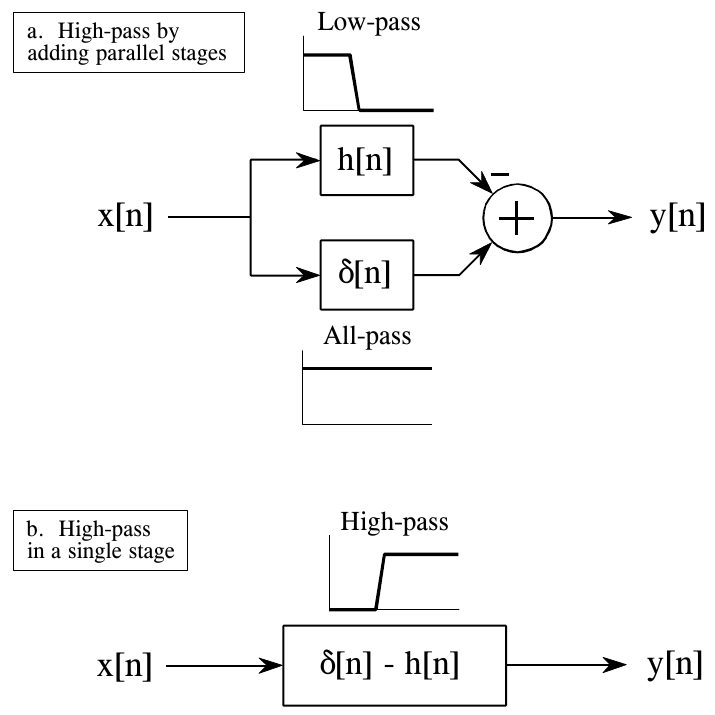
\includegraphics[width=0.596\linewidth,height=0.8\textheight,keepaspectratio]{assets/ch14/fig14-06.png}
\caption*{\textbf{图 14-6　频谱反转的框图。} 在 (a) 中，输入信号 x{[}n{]}
送入两个并联的系统，它们的冲激响应分别为 h{[}n{]} 和 δ{[}n{]}。如 (b)
所示，组合后系统的冲激响应为 δ{[}n{]} −
h{[}n{]}。这意味着组合系统的频率响应是 h{[}n{]} 频率响应的反转。 （a.
High-pass by adding parallel stages = 用并联相加的方式得到高通；b.
High-pass in a single stage = 单级高通；Low-pass = 低通，All-pass =
全通，High-pass = 高通；加法器上的 −
号表示减去该支路。原书这段图注排在图的左侧，裁图时已去掉，译文见上。）}
\end{figure}

这在计算机程序中可以分两步完成：让信号通过一个低通滤波器，再从原信号中减去滤波后的信号。不过，把两个滤波器核合并起来，整个操作可以在单级中完成。第
7 章讲过，输出相加的并联系统可以通过把冲激响应相加合并成单级。如 (b)
所示，高通滤波器的滤波器核为 δ{[}n{]} −
h{[}n{]}。也就是说，把所有采样的符号取反，再在对称中心的采样上加一。

\begin{quote}
\textbf{译注：} 原文此处写作 ``performed in a signal stage''，应为
``single stage''（单级），按后者译出。
\end{quote}

要让这个技巧奏效，从低通滤波器出来的低频成分，必须与从全通系统出来的低频成分相位相同，否则就无法完全相减。这给方法加上了两条限制：(1)
原滤波器核必须左右对称（即零相位或线性相位）；(2)
冲激必须加在对称中心处。

从低通到高通的第二种方法是频谱翻转，如图 14-7 所示。和前面一样，(a)
中的低通滤波器核对应 (b) 中的频率响应。把 (a)
中每隔一个的采样取反，就得到高通滤波器核 (c)。如 (d)
所示，这使频域左右翻转：0 变成 0.5，0.5 变成
0。示例低通滤波器的截止频率是 0.15，因此高通滤波器的截止频率是 0.35。

\begin{figure}[htbp]
\centering
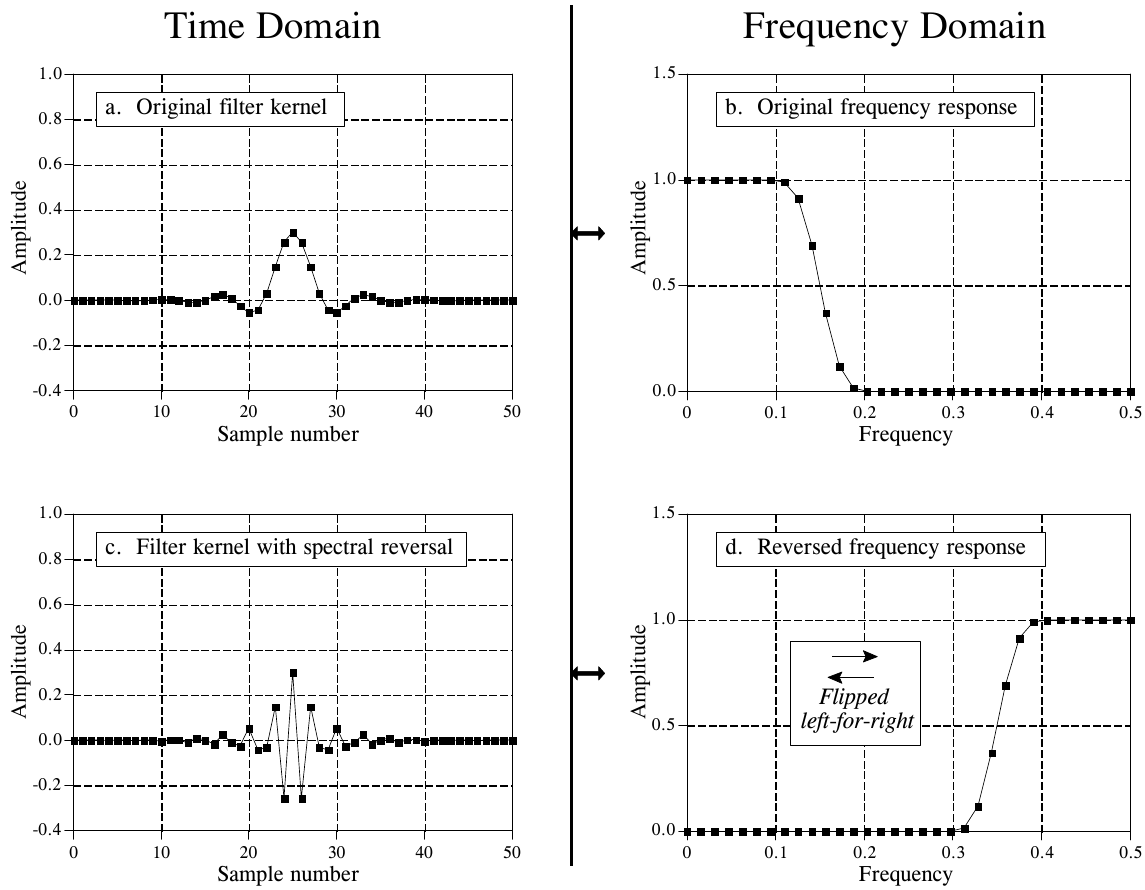
\includegraphics[width=0.954\linewidth,height=0.8\textheight,keepaspectratio]{assets/ch14/fig14-07.png}
\caption*{\textbf{图 14-7　频谱翻转的例子。} (a) 中低通滤波器核的频率响应如 (b)
所示。把 (a) 中每隔一个的采样取反，就得到高通滤波器核
(c)。时域中的这一操作使频域左右翻转，得到 (d) 所示的高通频率响应。
（Time Domain = 时域，Frequency Domain = 频域；a. Original filter kernel
= 原滤波器核；b. Original frequency response = 原频率响应；c.~Filter
kernel with spectral reversal = 频谱翻转后的滤波器核；d.~Reversed
frequency response = 翻转后的频率响应；Flipped left-for-right =
左右翻转。Amplitude = 幅度，Sample number = 采样序号，Frequency =
频率。）}
\end{figure}

把每隔一个的采样取反，等价于把滤波器核乘以一个频率为 0.5 的正弦波。第 10
章讲过，这会使频域平移 0.5。看着 (b)，想象 −0.5 到 0
之间的负频率，它们是 0 到 0.5 之间频率的镜像。(d) 中出现的频率，正是 (b)
中的负频率平移 0.5 之后的结果。

最后，图 14-8 和 14-9
展示了怎样把低通和高通滤波器核组合成带通和带阻滤波器。简单地说，把滤波器核相加得到带阻滤波器，把滤波器核卷积得到带通滤波器。这依据的是第
7
章讨论过的级联系统和并联系统的合并方式。这些技巧也可以多次组合使用。例如，可以先把两个滤波器核相加，构成一个带阻滤波器，再用前面讲的频谱反转或频谱翻转，就设计出了一个带通滤波器。所有这些技巧都非常好用，很少会有意外。

\begin{quote}
\textbf{译注：} 原文把相加得到的滤波器写作 ``stop-pass
filter''，按上下文就是带阻(band-reject)滤波器，译文直接译作带阻。
\end{quote}

\begin{figure}[htbp]
\centering
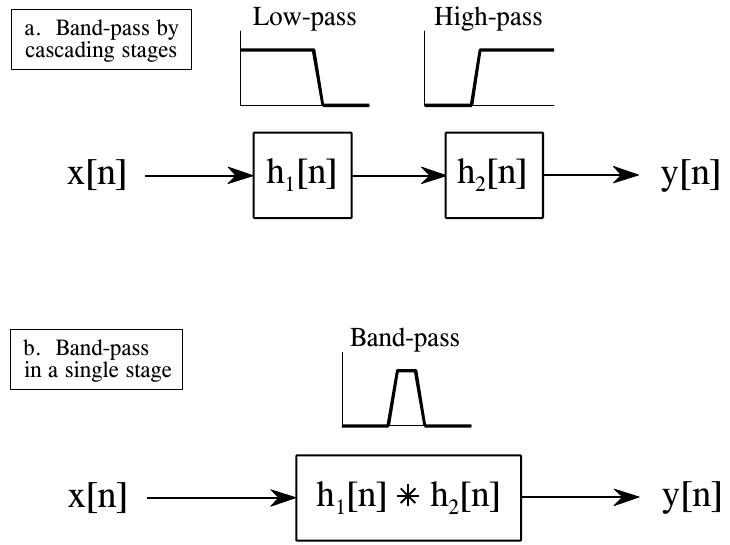
\includegraphics[width=0.608\linewidth,height=0.8\textheight,keepaspectratio]{assets/ch14/fig14-08.png}
\caption*{\textbf{图 14-8　设计带通滤波器。} 如 (a)
所示，把一个低通滤波器和一个高通滤波器级联，就能构成带通滤波器。这可以化简为
(b) 所示的单级，单级的滤波器核等于低通和高通滤波器核的卷积。 （a.
Band-pass by cascading stages = 用级联得到带通；b. Band-pass in a single
stage = 单级带通；Low-pass = 低通，High-pass = 高通，Band-pass =
带通；方框里的 \dspsym{∗}
是卷积。原书这段图注排在图的左侧，裁图时已去掉，译文见上。）}
\end{figure}

\begin{figure}[htbp]
\centering
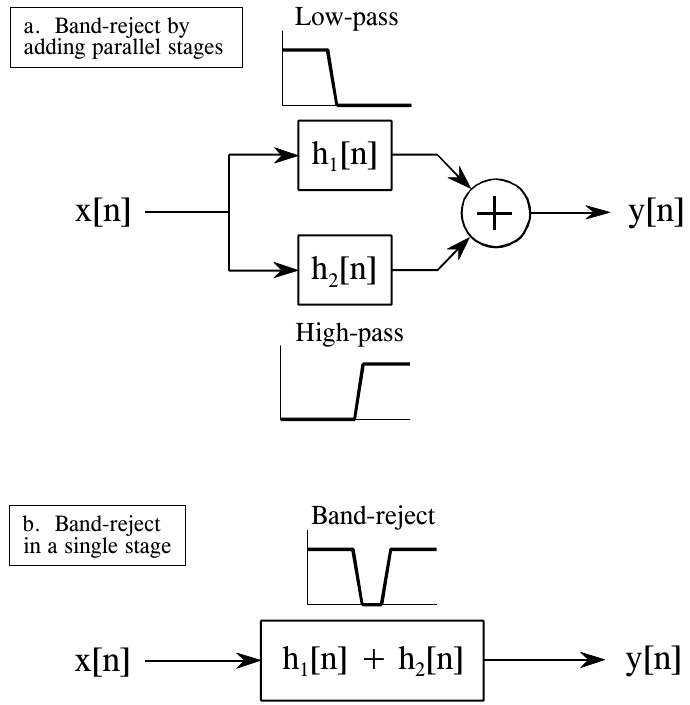
\includegraphics[width=0.575\linewidth,height=0.8\textheight,keepaspectratio]{assets/ch14/fig14-09.png}
\caption*{\textbf{图 14-9　设计带阻滤波器。} 如 (a)
所示，把一个低通滤波器和一个高通滤波器并联、输出相加，就构成带阻滤波器。图
(b) 是化简后的单级，其滤波器核等于低通和高通滤波器核之和。 （a.
Band-reject by adding parallel stages = 用并联相加得到带阻；b.
Band-reject in a single stage = 单级带阻；Low-pass = 低通，High-pass =
高通，Band-reject =
带阻。原书这段图注排在图的左侧，裁图时已去掉，译文见上。）}
\end{figure}

\section{滤波器的分类}

表 14-1
总结了数字滤波器怎样按用途和实现方式分类。数字滤波器的用途可分为三类：时域、频域和定制(custom)。如前所述，当信息编码在信号波形的形状中时，用时域滤波器。时域滤波用于平滑、去直流、波形整形等操作。相比之下，当信息包含在各正弦分量的幅度、频率和相位中时，用频域滤波器。这类滤波器的目标是把一个频带与另一个频带分开。当需要滤波器完成某种特殊操作、比四种基本响应（高通、低通、带通和带阻）更复杂的事情时，就用定制滤波器。例如，第
17
章介绍怎样用定制滤波器做反卷积(deconvolution)，这是抵消一次不想要的卷积的一种方法。

\textbf{表 14-1　滤波器的分类。} 滤波器可以按用途和实现方式划分。

{\def\LTcaptype{none} % do not increment counter
\begin{longtable}[]{@{}
  >{\raggedright\arraybackslash}p{(\linewidth - 4\tabcolsep) * \real{0.3333}}
  >{\raggedright\arraybackslash}p{(\linewidth - 4\tabcolsep) * \real{0.3333}}
  >{\raggedright\arraybackslash}p{(\linewidth - 4\tabcolsep) * \real{0.3333}}@{}}
\toprule\noalign{}
\begin{minipage}[b]{\linewidth}\raggedright
滤波器用于 ＼ 滤波器实现方式
\end{minipage} & \begin{minipage}[b]{\linewidth}\raggedright
卷积\\
有限冲激响应（FIR）\strut
\end{minipage} & \begin{minipage}[b]{\linewidth}\raggedright
递归\\
无限冲激响应（IIR）\strut
\end{minipage} \\
\midrule\noalign{}
\endhead
\bottomrule\noalign{}
\endlastfoot
\textbf{时域}（平滑、去直流） & 移动平均（第 15 章） & 单极点（第 19
章） \\
\textbf{频域}（分离频率） & 加窗 sinc（第 16 章） & 切比雪夫（第 20
章） \\
\textbf{定制}（反卷积） & FIR 定制（第 17 章） & 迭代设计（第 26 章） \\
\end{longtable}
}

（原表英文：FILTER USED FOR = 滤波器用于，FILTER IMPLEMENTED BY =
滤波器实现方式；Convolution = 卷积，Recursion = 递归；Moving average =
移动平均(moving average)，Single pole = 单极点(single
pole)，Windowed-sinc = 加窗 sinc，Chebyshev = 切比雪夫(Chebyshev)，FIR
custom = FIR 定制，Iterative design = 迭代设计(iterative design)。）

数字滤波器可以用两种方式实现：卷积（也叫有限冲激响应，FIR）和递归（也叫无限冲激响应，IIR）。用卷积实现的滤波器性能可以远好于用递归实现的滤波器，但执行起来慢得多。

接下来的六章按照表 14-1
的分类介绍数字滤波器。首先看用卷积实现的滤波器。移动平均（第 15
章）用于时域，加窗 sinc（第 16 章）用于频域，FIR 定制（第 17
章）用于需要特殊处理的场合。为了结束对 FIR 滤波器的讨论，第 18
章介绍一种叫 FFT 卷积的技术。这是一种提高卷积速度的算法，能让 FIR
滤波器执行得更快。

接着看递归滤波器。单极点递归滤波器（第 19
章）用于时域，而切比雪夫滤波器（第 20
章）用于频域。具有定制响应的递归滤波器要用迭代技术来设计。因此，我们把它们的讨论推迟到第
26 章，在那里和另一种迭代方法------神经网络(neural
network)------一起介绍。

如表 14-1
所示，卷积和递归是相互竞争的技术，在具体应用中你只能选其一。怎么选？第
21 章会在时域和频域两方面对二者做正面比较。
